\documentclass{article}
\usepackage[T1]{fontenc}
\usepackage{lmodern}
\usepackage{graphicx}
\usepackage{amsmath,amssymb}
\usepackage[a4paper,margin=2cm]{geometry}
\usepackage[absolute,overlay]{textpos}
\setlength{\TPHorizModule}{1mm}
\setlength{\TPVertModule}{1mm}
\usepackage[indonesian]{babel}
\usepackage{hyperref}
\setlength{\emergencystretch}{2em}
% unit: Halaman 47

\begin{document}

% === Halaman 47 (llm) ===

\vspace{68.31mm}

(a) Enkripsi
\vspace{60mm}
(b) Dekripsi

\vspace{98.01mm}

% deskripsi: Diagram alur proses enkripsi menggunakan Counter Mode (CTR), menunjukkan input Counter, Kunci (K), Plaintext (P) yang di-XOR dengan output enkripsi E untuk menghasilkan Ciphertext (C).
% bbox normalisasi: [0.2200, 0.2000, 0.8800, 0.4300]
\begin{textblock*}{138.60mm}(46.20mm,59.40mm)
\noindent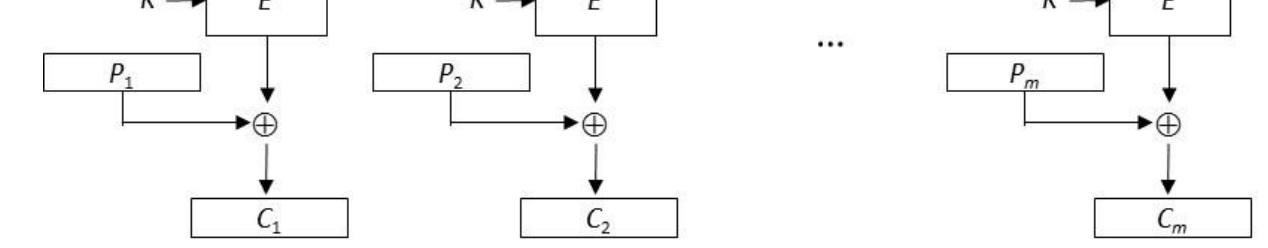
\includegraphics[width=138.60mm,height=68.31mm]{../../images/llm/page_047_img_01.png}%
\end{textblock*}

% deskripsi: Diagram alur proses dekripsi menggunakan Counter Mode (CTR), menunjukkan input Counter, Kunci (K), dan Ciphertext (C) yang di-XOR dengan output enkripsi E untuk mengembalikan Plaintext (P).
% bbox normalisasi: [0.2200, 0.5300, 0.8800, 0.8600]
\begin{textblock*}{138.60mm}(46.20mm,157.41mm)
\noindent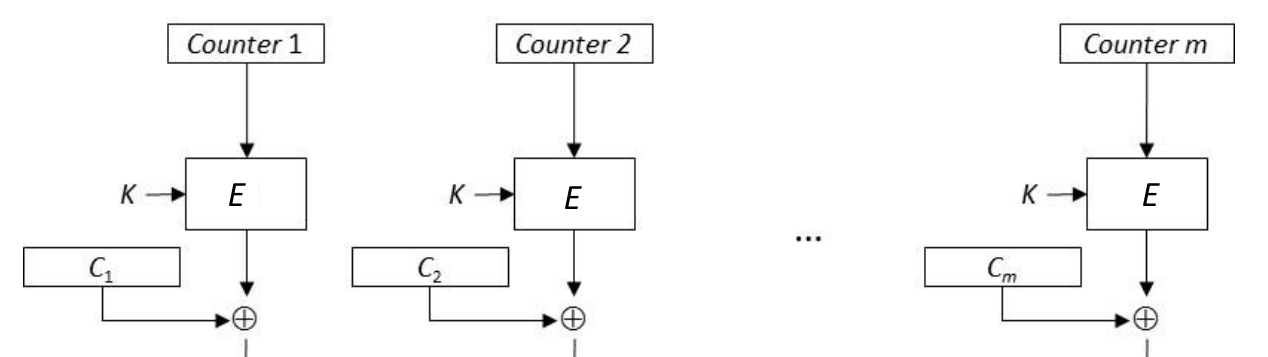
\includegraphics[width=138.60mm,height=98.01mm]{../../images/llm/page_047_img_02.png}%
\end{textblock*}

\end{document}
